% !TeX root = ../master.tex

\lecture{6}{2026-09-29}{Convection, Pt. II}

\section{External Forced Convection}

\subsection{Parallel Flow over Flat Plates}
We consider the parallel flow of a fluid over a flat plate of length $L$ in the flow direction as shown in \mref{fig:flatplateflow}.
Here, the $x$-coordinate is measured along the plate surface from the leading edge in the flow-direction.
The fluid approaches the plate in the $x$-direction with a uniform velocity $V$ and temperature $T_{\infty}$.
The flow in the boundary layer is initially laminar, but becomes turbulent at a distance $x_{\mathrm{cr}}$ from the leading edge where the Reynolds number reaches its critical value for transition -- For flow over a flat plate transition occurs at about $\mathrm{Re} \approx \num{5e5}$ \citepage{cengel2015heatmasstransfer}{428--429}.

\begin{figure} [ht]
  \centering
  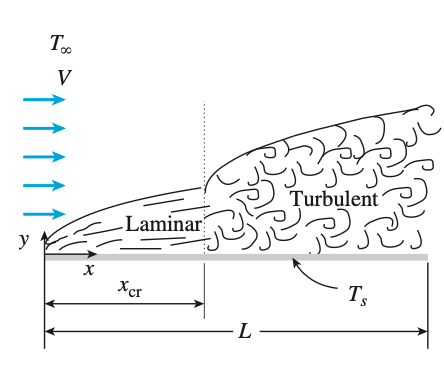
\includegraphics[width=0.5\linewidth]{./figures/flatplateflow.png}
  \caption{Laminar and turbulent flowregions of the boundary layer during flow over a flat plate. Reproduced from \citepage{cengel2015heatmasstransfer}{Fig.~7--6}.}
  \label{fig:flatplateflow}
\end{figure}

\subsubsection{Friction Coefficient}
For laminar flow over a plate the boundary layer coefficient is analytically determined to be \citepage{cengel2015heatmasstransfer}{Eq.~(7--12a, b)}:
\begin{equation} \label{eq:laminarfriction}
  \delta = \frac{\num{4,91} x}{\sqrt{\mathrm{Re}_x}}, \quad C_{f,x} = \frac{\num{0,664} }{\sqrt{\mathrm{Re}_x}}, \quad \mathrm{Re}_x < \num{5e5} 
.\end{equation}
From experiments the corresponding relations for turbulent flow are found to be \citepage{cengel2015heatmasstransfer}{Eq.~(7--13a, b)}
\begin{equation} \label{eq:turbulentfriction}
  \delta = \frac{\num{0,38} x}{\sqrt[5]{\mathrm{Re}_x}}, \quad C_{f,x} = \frac{\num{0,059} }{\sqrt[5]{\mathrm{Re}_x}}, \quad \num{5e5} \leq \mathrm{Re}_x \leq \num{e7}
.\end{equation}
Note the local friction coefficient $C_{f,x} \propto \mathrm{Re}_x^{- 1 / 2}$ and thus to $x^{- 1 / 2}$ for laminar flow.
Hence, $C_{f,x}$ is supposedly infinite at the leading edge and decreases by a factor of $x^{- 1 / 2}$ in the flow direction.
Also, note that $C_{f,x}$ reaches its highest value when the flow turns fully turbulent, where after it decreases by a factor of $x^{- 1 / 5}$ in the flow direction.

The average friction coefficient over the entire surface is then found using integration over the entire length \citepage{cengel2015heatmasstransfer}{Eq.~(7--7)}
\begin{equation} \label{eq:avgfriction}
  C_f = \frac{1}{L} \int_{0}^{L} C_{f,x} \, \mathrm{d}x
.\end{equation}
Substituting \mref{eq:laminarfriction} and \mref{eq:turbulentfriction} into \mref{eq:avgfriction} and performing the integration we obtain \citepage{cengel2015heatmasstransfer}{Eqs.~(7--14)--(7--15)}
\begin{align}
  \text{Laminar:}& & C_f &= \frac{\num{1,33}}{\sqrt{\mathrm{Re}_L}}, & \mathrm{Re}_L &< \num{5e5}  \label{eq:laminarfrictioncoeff} \\
  \text{Turbulent:}& & C_f &= \frac{\num{0,074}}{\sqrt[5]{\mathrm{Re}_L}}, & \num{5e5} \leq \mathrm{Re}_L &\leq \num{e7} \label{eq:turbulentfrictioncoeff}
.\end{align}
\Mref{eq:laminarfrictioncoeff} gives the average friction coefficient for the entire plate when the flow is laminar over the entire plate, note that this is twice the value of the local friction coefficient at the end of the plate, $C_f = 2 C_{f,x=L}$.
\Mref{eq:turbulentfrictioncoeff} gives the average friction over the entire plate when the flow is turbulent over the entire plate or when the laminar flow region is small enough to be neglected $x_{\mathrm{cr}} \ll L$.

To obtain the actual friction coefficient over a plate with both a laminar and turbulent region, the integration in \mref{eq:avgfriction} is carried out over the laminar region using \mref{eq:laminarfriction} and the turbulent region using \mref{eq:turbulentfriction} as \citepage{cengel2015heatmasstransfer}{Eq.~(7--16)}
\begin{equation} \label{eq:frictioncoeffplate}
  C_f = \frac{1}{L} \left( \int_{0}^{x_{\mathrm{cr}}} C_{f,x, \text{laminar}} \, \mathrm{d}x  + \int_{x_{\mathrm{cr}}}^{L} C_{f, x, \text{turbulent}} \, \mathrm{d}x  \right)
.\end{equation}
Taking the critical Reynolds number to be $\mathrm{Re}_{\mathrm{cr}} = \num{5e5}$ the integration in \mref{eq:frictioncoeffplate} is solved to obtain the following expression for the average friction coefficient over the entire plate
\begin{equation} \label{eq:frictioncoeffplatesimplified}
  C_f = \frac{\num{0,074} }{\sqrt[5]{\mathrm{Re}_L}} - \frac{1742}{\mathrm{Re}_L}, \quad \num{5e5} \leq \mathrm{Re}_L \leq \num{e7} 
.\end{equation}
In \mref{eq:frictioncoeffplatesimplified} the surfaces are assumed to be smooth and the free stream is assumed turbulence tree.

For laminar flow, the friction coefficient only depends on Reynolds number, whereas for turbulent flow, surface roughness causes the friction coefficient to increase many times.
Experimental observations give a average friction coefficient for turbulent flow over rough surfaces as:
\begin{equation*}
  C_f = \left( \num{1,89} - \num{1,62} \log \frac{\epsilon}{L} \right)^{-\num{2,5}}
,\end{equation*}
where $\epsilon$ is the surface roughness and $L$ is the length of the plate in the flow direction.
This relation is applicable for turbulent flow on rough surfaces for $\mathrm{Re} > \num{e6}$ especially when $\epsilon / L > \num{e-4}$ \citepage{cengel2015heatmasstransfer}{429--430}.

\subsubsection{Heat Transfer Coefficient}
The locals Nusselt number at a location $x$ for laminar flow over a flat plate can be found analytically by solving the differential energy equation to be \citepage{cengel2015heatmasstransfer}{Eq.~(7--19)}
\begin{equation*}
  \mathrm{Nu}_x = \frac{h_x x}{k} = \num{0,332} \sqrt{\mathrm{Re}_x} \sqrt[3]{\mathrm{Pr}}, \quad \mathrm{Pr} > \num{0,6}, \mathrm{Re}_x < \num{5e5}.
.\end{equation*}
From experiments, the corresponding relation for turbulent flow is \citepage{cengel2015heatmasstransfer}{Eq.~(7--20)}
\begin{equation*}
  \mathrm{Nu}_x = \frac{h_x x}{k} = \num{0,0296} \mathrm{Re}_x^{\num{0,8}} \sqrt[3]{\mathrm{Pr}}, \quad \num{0,6} \leq \mathrm{Pr} \leq \num{60}, \num{5e5} \leq \mathrm{Re}_x \leq \num{e7}
.\end{equation*}
Like, for the friction coefficient $h_x$ is, for laminar flow, proportional to $\sqrt{\mathrm{Re}_x}$ and thus to $x^{-1 / 2}$, meaning $h_x$ is supposedly infinite at the leading edge and decreases by a factor of $x^{- 1 / 2}$ in the flow direction.

Like for the friction coefficient the average convection coefficient over the entire surface is found through integration \citepage{cengel2015heatmasstransfer}{Eq.~(7--8)}
\begin{equation*}
  h = \frac{1}{L} \int_{0}^{L} h_x \, \mathrm{d}x 
.\end{equation*}
Hence, the average Nusselt number over the entire plate is \citepage{cengel2015heatmasstransfer}{Eqs.~(7--21)--(7--22)}
\begin{align}
  \text{Laminar:}& & \mathrm{Nu} &= \frac{h L}{k} = \num{0,664} \sqrt{\mathrm{Re}_L} \sqrt[3]{\mathrm{Pr}}, & \mathrm{Re}_L < \num{5e5}&, \mathrm{Pr} > \num{0,6}    \\
  \text{Turbulent:}& & \mathrm{Nu} &= \frac{h L}{k} = \num{0,037} \mathrm{Re}_L^{\num{0,8} } \sqrt[3]{\mathrm{Pr}}, & \num{5e5} \leq \mathrm{Re}_L \leq \num{e7}&, \num{0,6} \leq \mathrm{Pr} \leq \num{60} 
.\end{align}
Here, the same conditions apply as for the friction coefficient in that the laminar result only applies for fully laminar flow and vice versa for the turbulent result.
An accurate heat transfer coefficient can be found by performing the same integration as for the friction coefficient.
Taking the critical Reynolds number to be $\mathrm{Re}_{\mathrm{cr}} = \num{5e5} $ the resulting average Nusselt number over the entire plate is \citepage{cengel2015heatmasstransfer}{Eq.~(7--24)}
\begin{equation*}
  \mathrm{Nu} = \frac{h L}{k} = \left( \num{0,037} \mathrm{Re}_L^{\num{0,8} } - \num{871} \right) \sqrt[3]{\mathrm{Pr}}, \quad \num{0,6} \leq \mathrm{Pr} \leq \num{60}, \num{5e5} \leq \mathrm{Re}_L \leq \num{e7} 
.\end{equation*}
Using curve-fitting the following relation for the Nusselt number, which is claimed to be applicable for all Prandtl numbers with an accuracy of $\pm \qty{1}{\percent}$ \citepage{cengel2015heatmasstransfer}{Eq.~(7--26); pp.~430--432}
\begin{equation*}
  \mathrm{Nu}_x = \frac{h_c x}{k} = \frac{\num{0,3387} \sqrt[3]{\mathrm{Pr}} \sqrt{\mathrm{Re}_x}}{\sqrt[4]{1 + \left( \num{0,0468} / \mathrm{Pr} \right)^{2 / 3}}}, \qquad \mathrm{Re}_x \mathrm{Pr} \geq \num{100}
.\end{equation*}

\subsection{Flow Across Cylinders and Spheres}
The characteristic length for a circular cylinder or sphere is the external diameter $D$.
Thus, the Reynolds number for a circular cylinder or sphere is $\mathrm{Re} = \mathrm{Re}_D = V D / \nu$, where $V$ is the velocity as it approaches the cylinder or sphere.
The critical Reynolds number for flow across a circular cylinder or sphere is about $\mathrm{Re}_{\mathrm{cr}} \approx \num{2e5} $ \citepage{cengel2015heatmasstransfer}{438}.

\subsubsection{Heat Transfer Coefficient}
Flows across cylinders and spheres generally involve flow separation and are thus difficult to analyze analytically.
Hence, such flows much be studied experimentally or numerically.
The average Nusselt number for cross flow over a cylinder is given by \citepage{cengel2015heatmasstransfer}{Eq.~(7--35)}
\begin{equation*}
  \mathrm{Nu}_{\mathrm{cyl}} = \frac{h D}{k} = \num{0,3} + \frac{\num{0,62} \sqrt{\mathrm{Re}} \sqrt[3]{\mathrm{Pr}}}{\sqrt[4]{1 + \left( \num{0,4} / \mathrm{Pr} \right)^{2 / 3}}} \left( 1 + \left( \frac{\mathrm{Re}}{\num{282000}} \right)^{5 / 8} \right)^{4 / 5}
.\end{equation*}
For flow over a sphere, the average Nusselt number is \citepage{cengel2015heatmasstransfer}{Eq.~(7--36)}
\begin{gather*}
  \mathrm{Nu}_{\mathrm{sph}} = \frac{h D}{k} = 2 + \left( \num{0,4} \sqrt{\mathrm{Re}} + \num{0,06} \mathrm{Re}^{2 / 3} \right) \mathrm{Pr}^{\num{0,4}} \sqrt[4]{\frac{\mu_{\infty}}{\mu_s}}, \\
  \num{3,5} \leq \mathrm{Re} \leq \num{8e4}, \quad \num{0,7} \leq \mathrm{Pr} \leq \num{380}, \quad \num{1,0} \leq \mu_{\infty} / \mu_s \leq \num{3,2}
.\end{gather*}
All the fluid properties in this case are evaluated at the free-stream temperature $T_{\infty}$, except for $\mu_s$, which is evaluated at the surface temperature $T_s$.

The average Nusselt number for flow across cylinders can be expressed compactly as \citepage{cengel2015heatmasstransfer}{Eq.~(7--37)}
\begin{equation*}
  \mathrm{Nu}_{\mathrm{cyl}} = \frac{h D}{k} = C \mathrm{Re}^{m} \mathrm{Pr}^{n}
,\end{equation*}
where $n = 1 / 3$ and the experimentally determined constants $C$ and $m$ are given in \mref{tab:nusselt-crossflow-cylinders} \citepage{cengel2015heatmasstransfer}{442--443}.

\begin{table}[htbp]
  \centering
  \caption{Empirical correlations for the average Nusselt number for forced
    convection over circular and noncircular cylinders in crossflow.
    Adapted from \citepage{cengel2015heatmasstransfer}{Tab.~7--1}.}
  \label{tab:nusselt-crossflow-cylinders}
  \small
  \begin{tabularx}{\linewidth}{
    @{}
    >{\raggedright\arraybackslash}p{0.21\linewidth}
    >{\raggedright\arraybackslash}p{0.13\linewidth}
    >{\raggedright\arraybackslash}p{0.19\linewidth}
    >{\raggedright\arraybackslash}X
    @{}
  }
    \toprule
    Cross-section of cylinder & Fluid & Range of $\mathrm{Re}$ & Nusselt number \\
    \midrule

    Circle
      & Gas or liquid
      & \makecell[l]{%
        \numrange{0,4}{4} \\
        \numrange{4}{40} \\
          \numrange{40}{4000} \\
          \numrange{4000}{40000} \\
        \numrange{40000}{400000}}
      & \makecell[l]{%
          $\mathrm{Nu}=\num{0,989} \mathrm{Re}^{\num{0,330}}\mathrm{Pr}^{1/3}$\\
          $\mathrm{Nu}=\num{0,911} \mathrm{Re}^{\num{0,385} }\mathrm{Pr}^{1/3}$\\
          $\mathrm{Nu}=\num{0,683} \mathrm{Re}^{\num{0,466} }\mathrm{Pr}^{1/3}$\\
          $\mathrm{Nu}=\num{0,193} \mathrm{Re}^{\num{0,618} }\mathrm{Pr}^{1/3}$\\
          $\mathrm{Nu}=\num{0,027} \mathrm{Re}^{\num{0,805} }\mathrm{Pr}^{1/3}$}
    \\
    \midrule

    Square
      & Gas
      & \numrange{3900}{79000} 
      & $\mathrm{Nu}=\num{0,094} \mathrm{Re}^{\num{0,675} }\mathrm{Pr}^{1/3}$
    \\
    \midrule

    Square, tilted \qty{45}{\degree} 
      & Gas
      & \numrange{5600}{111000} 
      & $\mathrm{Nu}=\num{0,258} \mathrm{Re}^{\num{0,588} }\mathrm{Pr}^{1/3}$
    \\
    \midrule

    Hexagon
      & Gas
      & \numrange{4500}{90700} 
      & $\mathrm{Nu}=\num{0,148} \mathrm{Re}^{\num{0,638} }\mathrm{Pr}^{1/3}$
    \\
    \midrule

    Hexagon, tilted $45^\circ$
      & Gas
      & \makecell[l]{%
      \numrange{5200}{20400} \\
      \numrange{20400}{105000} }
      & \makecell[l]{%
          $\mathrm{Nu}=\num{0,162} \mathrm{Re}^{\num{0,638} }\mathrm{Pr}^{1/3}$\\
          $\mathrm{Nu}=\num{0,039} \mathrm{Re}^{\num{0,782} }\mathrm{Pr}^{1/3}$}
    \\
    \midrule

    Vertical plate
      & Gas
      & \numrange{6300}{23600} 
      & $\mathrm{Nu}=\num{0,257} \mathrm{Re}^{\num{0,731} }\mathrm{Pr}^{1/3}$
    \\
    \midrule

    Ellipse
      & Gas
      & \numrange{1400}{8200} 
      & $\mathrm{Nu}=\num{0,197} \mathrm{Re}^{\num{0,612} }\mathrm{Pr}^{1/3}$
    \\

    \bottomrule
  \end{tabularx}
\end{table}

\subsubsection{Flow Across Tube Banks}
Flow through tube banks is studied experimentally as it is too complex to be treated analytically.
The average Nusselt number over the entire tube bank is \citepage{cengel2015heatmasstransfer}{Eq.~(7--42)}
\begin{equation*}
  \mathrm{Nu}_D = \frac{h D}{k} C \mathrm{Re}_D^{m} \mathrm{Pr}^{n} \sqrt[4]{\mathrm{Pr} / \mathrm{Pr}_s}
,\end{equation*}
where $D$ is the tube diameter and the values of the constants $C$, $m$, and $n$ depend on the Reynolds number.
Such correlations are given in \mref{tab:nusselt-tube-banks} for tube banks with more than \num{16} rows $N_L > 16$, $\num{0,7} < \mathrm{Pr} < \num{500}$ and $0 < \mathrm{Re}_D < \num{2e6} $ with an uncertainty of $\pm \qty{15}{\percent}$.
Note that all properties except $\mathrm{Pr}_s$ are evaluated at the arithmetic mean temperature $T_m$ of the fluid determined from \citepage{cengel2015heatmasstransfer}{Eq.~(7--43)}
\begin{equation*}
  T_m = \frac{T_i + T_e}{2}
\end{equation*}
where $T_i$ and $T_e$ are the fluid inlet and exit temperatures of the tube bank respectively.

The average Nusselt number relations given in \mref{tab:nusselt-tube-banks} are only applicable for tube banks with more than \num{16} rows.
These relations can also be used for tube banks with $N_L < \num{16}$ provided they are modified using \citepage{cengel2015heatmasstransfer}{Eq.~(7--44)}
\begin{equation} \label{eq:corneeded}
  \mathrm{Nu}_{D, N_{L < \num{16} }} = F \mathrm{Nu}_D
,\end{equation}
where $F$ is a correction factor whose values are given in \mref{tab:tube-bank-correction-factor}.
For $\mathrm{Re}_D > \num{1000}$ the correction factor is independent of Reynolds number. 



\begin{table}[htbp]
  \centering
  \caption{Nusselt number correlations for crossflow over tube banks for
  $N_L > \num{16}$ and $\num{0,7}  < \mathrm{Pr} < \num{500} $. Adapted from \citepage{cengel2015heatmasstransfer}{Tab.~7--2}.}
  \label{tab:nusselt-tube-banks}
  \small
  \begin{tabularx}{\linewidth}{
    @{}
    >{\raggedright\arraybackslash}p{0.17\linewidth}
    >{\raggedright\arraybackslash}p{0.22\linewidth}
    >{\raggedright\arraybackslash}X
    @{}
  }
    \toprule
    Arrangement & Range of $\mathrm{Re}_D$ & Correlation \\
    \midrule

    \multirow{4}{*}{In-line}
                & \numrange{0}{100} 
      & $\mathrm{Nu}_D = \num{0,9}\mathrm{Re}_D^{\num{0,4} } \mathrm{Pr}^{\num{0,36} }(\mathrm{Pr}/\mathrm{Pr}_s)^{\num{0,25} }$ \\
      & \numrange{100}{1000} 
      & $\mathrm{Nu}_D = \num{0,52} \mathrm{Re}_D^{\num{0,5} } \mathrm{Pr}^{\num{0,36} }(\mathrm{Pr}/\mathrm{Pr}_s)^{\num{0,25} }$ \\
      & \numrange{1000}{2e5} 
      & $\mathrm{Nu}_D = \num{0,27} \mathrm{Re}_D^{\num{0,63} } \mathrm{Pr}^{\num{0,36} }(\mathrm{Pr}/\mathrm{Pr}_s)^{\num{0,25} }$ \\
      & \numrange{2e5}{2e6} 
      & $\mathrm{Nu}_D = \num{0,033}\mathrm{Re}_D^{\num{0,8} } \mathrm{Pr}^{\num{0,4} }(\mathrm{Pr}/\mathrm{Pr}_s)^{\num{0,25} }$ \\
    \midrule

    \multirow{4}{*}{Staggered}
      & \numrange{0}{500} 
      & $\mathrm{Nu}_D = \num{1,04}\mathrm{Re}_D^{\num{0,4} }\mathrm{Pr}^{\num{0,36} }(\mathrm{Pr}/\mathrm{Pr}_s)^{\num{0,25} }$ \\
      & \numrange{500}{1000} 
      & $\mathrm{Nu}_D = \num{0,71}\mathrm{Re}_D^{0.5} \mathrm{Pr}^{0.36}(\mathrm{Pr}/\mathrm{Pr}_s)^{0.25}$ \\
      & \numrange{1000}{2e5} 
      & $\mathrm{Nu}_D = \num{0,35} (S_T/S_L)^{\num{0,2} } \mathrm{Re}_D^{\num{0,6} }\mathrm{Pr}^{\num{0,36} } (\mathrm{Pr}/\mathrm{Pr}_s)^{\num{0,25} }$ \\
      &  \numrange{2e5}{2e6} 
      & $\mathrm{Nu}_D = \num{0,031} (S_T/S_L)^{\num{0,2} } \mathrm{Re}_D^{\num{0,8} }\mathrm{Pr}^{\num{0,36} } (\mathrm{Pr}/\mathrm{Pr}_s)^{\num{0,25} }$ \\
    \bottomrule
  \end{tabularx}
\end{table}

\begin{table}[htbp]
  \centering
  \caption{Correction factor $F$ for use in \mref{eq:corneeded} for $N_L<16$ and
    $\mathrm{Re}_D>1000$. Adapted from  \citepage{cengel2015heatmasstransfer}{Tab.~7--3}.}
  \label{tab:tube-bank-correction-factor}
  \begin{tabular}{@{}l*{8}{c}@{}}
    \toprule
    $N_L$ & \num{1}  & \num{2}  & \num{3}  & \num{4}  & \num{5}  & \num{7}  & \num{10}  & \num{13}  \\
    \midrule
    In-line   & \num{0,70}  & \num{0,80}  & \num{0,86}  & \num{0,90}  & \num{0,93}  & \num{0,96}  & \num{0,98}  & \num{0,99}  \\
    Staggered & \num{0,64}  & \num{0,76}  & \num{0,84}  & \num{0,89}  & \num{0,93}  & \num{0,96}  & \num{0,98}  & \num{0,99}  \\
    \bottomrule
  \end{tabular}
\end{table}

Once the Nusselt number and therefore the heat transfer coefficient for the entire tube bank is known, the heat transfer rate can be determined from Newton's law of cooling using a suitable temperature difference $\Delta T$.
This suitable temperature difference is, for internal flow, the log mean temperature difference $\Delta T_{1m}$ defined as \citepage{cengel2015heatmasstransfer}{Eq.~(7--45)}
\begin{equation*}
  \Delta T_{1m} = \frac{\left( T_s - T_e \right) - \left( T_s - T_i \right)}{\ln \left( \frac{T_s - T_e}{T_s - T_i} \right)} = \frac{\Delta T_e - \Delta T_i}{\ln \left( \frac{\Delta T_e}{\Delta T_i} \right)}
.\end{equation*}
Also, the exit temperature of the fluid $T_e$ can be determined from \citepage{cengel2015heatmasstransfer}{Eq.~(7--46)}
\begin{equation*}
  T_e = T_s - \left( T_s - T_i \right) \exp \left( - \frac{A_s h}{\dot{m} c_p} \right)
,\end{equation*}
where $A_s = N \pi D L$ is the heat transfer surface area and $\dot{m} = \rho V N_t S_T L$ is the mass flow rate of the fluid.
Here, $N$ is the total number of tubes in the bank, i.e. the product of $N_T$ and $N_L$ which are the number of tubes in the transverse plane and longitudinal plane respectively, $L$ is the length of the tubes, and $V$ is the velocity of the fluid just before entering the tube bank.
The heat transfer rate can be determined from \citepage{cengel2015heatmasstransfer}{Eq.~(7--47)}
\begin{equation*}
  \dot{Q} = h A_s \Delta T_{1m} = \dot{m} c_p \left( T_e - T_i \right)
.\end{equation*}
In the above the second relation is usually more convenient as it does not require the calculation of $\Delta T_{1m}$ \citepage{cengel2015heatmasstransfer}{446--449}.
